\documentclass[a4paper,12pt, twoside]{article}
%\documentclass[a4paper,12pt, twoside]{book}

\usepackage[papersize={210mm,297mm},tmargin=20mm,bmargin=20mm,lmargin=20mm,rmargin=20mm]{geometry}

\usepackage[utf8]{inputenc}
%https://mirror.hmc.edu/ctan/macros/latex/contrib/babel-contrib/turkish/turkish.pdf
\usepackage[english]{babel}
%\usepackage[T1]{fontenc}

\usepackage{amsmath,amssymb,mathabx}%\for eqref
\usepackage{lscape}

\usepackage{hyperref}
\hypersetup{
    colorlinks,
    citecolor=black,
    filecolor=black,
    linkcolor=blue,
    urlcolor=red}
  

%%% \usepackage{svg}
%%% https://tex.stackexchange.com/questions/122871/include-svg-images-with-the-svg-package/129854
\usepackage{graphicx}
\graphicspath{ {./figurler/} }

\usepackage[colorinlistoftodos]{todonotes}
\usepackage{fancyhdr}

\usepackage{indentfirst}
%% paragraf girintisi
\setlength{\parindent}{5ex}

%% Daha sonra yazılacak kısımları not düşmek için...
\newcommand{\YAZILACAK}{{\vspace{18pt}\bf\Large \color{red} YAZILACAK}}


\pagestyle{fancy}
\fancyhf{}
\lhead{ Kuantum Fiziği }
\chead{\thepage}
\rhead{Mesut Karakoç}
\lfoot{Akdeniz Üniversitesi}
\cfoot{}
%\rfoot{BF}

\title{Akdeniz Üniversitesi\\ Fen Fakültesi - Fizik Bölümü\\FİZ319 Kuantum Fiziği Ders Notları}

\author{\setlength{\unitlength}{6mm}
\begin{picture}(10,10)
\put(1.1,0){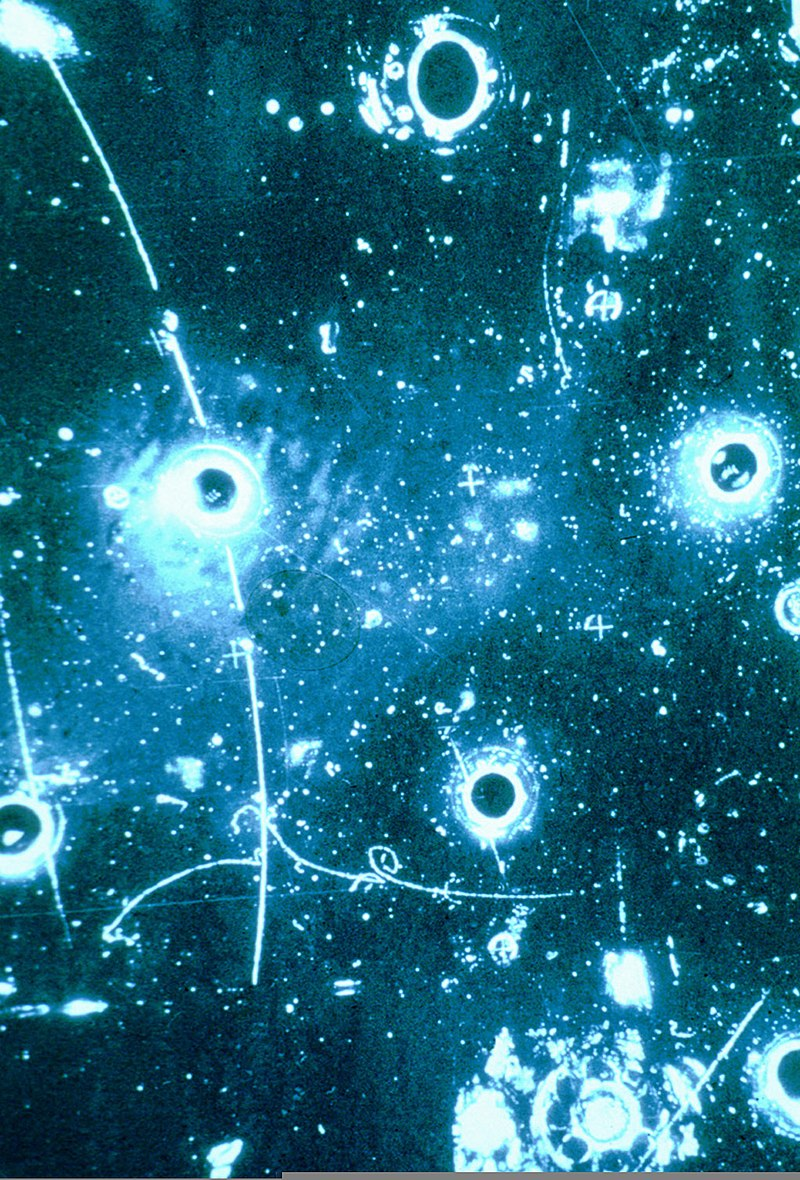
\includegraphics[width=4.5cm]{Leptonic_event_in_Gargamelle_bubble_chamber.jpg}}
\end{picture} \\ Doç. Dr. Mesut Karakoç}


\date{\today}

\begin{document}

%% Turkish babel problem
%% https://tex.stackexchange.com/questions/160385/newgeometry-doesnt-work-with-turkish-babel-package
%%\shorthandoff{=}% Make = not active any more

\maketitle

\newpage

% change name to "İçindekiler"
\renewcommand{\contentsname}{İçindekiler}
\tableofcontents{}

\listoffigures
 
\listoftables

\newpage

{
\hspace{.5\textwidth}
\begin{minipage}{.5\textwidth}
\raggedleft
If all this damned quantum jumps were really to stay, I should be
sorry I ever got involved with quantum theory.

—Erwin Schrödinger
\cite{book:Ficek}

%% Latince için
%% post iacturam quis non sapit!
%% Who is not wise after he has lost something?
%% https://quizlet.com/23756827/latin-proverbs-h-flash-cards/
\end{minipage}
}

\setcounter{section}{2} %% THIS WILL BE DELETED when all chapters merged!
\section{Schrödinger Denkleminin Ayrıştırılması, Özdeğerleri ve Özfonksiyonları}

Bu bölümde bir parçacığın veya sistemin etkisinde olduğu potansiyelin $V(x)$ zamandan bağımsız olması halinde, Schrödinger denkleminin sadece konum ve sadece zaman değişkenlerini içeren iki çiftlenmiş denklem seti halinde yazılabileceğini göreceğiz. Sadece konum değişkenine bağlı olarak yazılan yeni denklemi zamandan bağımsız Schrödinger denklemi olarak adlandırıyoruz. Devamında zamandan bağımsız denklem için özdeğer, özfonksiyon kavramlarını tartışacağız ve bazı potansiyeller için bu denklemin çözümlerini inceleyeceğiz. 

\subsection{Zamandan Bağımsız Schrödinger Denklemi}
%%
Bir önceki bölümde elde ettiğimiz zamana bağlı Schrödinger denklemini \emph{Hamilton} işlemcisini kullanarak,
%%
\begin{equation}
\hat H \psi ( x , t ) = i \hbar \frac { \partial \psi ( x , t ) } { \partial t }
\label{eq:time_depended_schrodinger_eq_op_form}
\end{equation}
%%
şeklinde yazabileceğimizi ve dalga fonksiyonlarıyla açık halini de, 
%%
\begin{equation}
- \frac { \hbar ^ { 2 } } { 2 m } \frac { \partial ^ { 2 } \psi ( x , t ) } { \partial x ^ { 2 } } + V ( x ) \psi ( x , t ) = i \hbar \frac { \partial \psi ( x , t ) } { \partial t }
\label{eq:time_depended_schrodinger_eq}
\end{equation}
%%
şeklinde yazabileceğimizi görmüştük.  Yukarıda tekrar yazdığımız zamana bağlı Schrödinger denklemi  bir kısmi diferansiyel denklemdir.  Kısmi diferansiyel denklemlerin birden çok bağımsız değişkenleri olur.   Bu nedenle genellikle  kısmi diferansiyel denklemleri çözmek kolay olmayabilir.  Fakat bizim inceleyeceğimiz durumda V(x)  potansiyeli zamandan bağımsız olduğundan denklemi sadece zamanı ve sadece konuma bağlı iki adi diferansiyel denkleme    dönüştürebiliriz. 
%%
\begin{equation}
\psi ( x , t ) = T ( t ) u ( x )
\label{eq:separation_of_wave_func}
\end{equation}

Bu dönüşümü gerçekleştirebilmek için $\psi ( x , t )$'nin yukarıdaki gibi iki fonksiyonun çarpımı şeklinde yazılabileceğini kabul edeceğiz. Dalga fonksiyonunun bu halin zamana bağlı Schrödinger denkleminde kullanırsak,
%%
\begin{equation*}
i \hbar u ( x ) \frac { d T ( t ) } { d t } = \left\{ - \frac { \hbar ^ { 2 } } { 2 m } \frac { d ^ { 2 } u ( x ) } { d x ^ { 2 } } + V ( x ) u ( x ) \right\} T ( t )
\end{equation*}
%%
denklemine ulaşırız. Bu denklemin her iki tarafını $T ( t ) u ( x )$ ifadesine bölersek,
%%
\begin{equation}
i \hbar \frac { 1 } { T ( t ) } \frac { d T ( t ) } { d t } = \frac { 1 } { u ( x ) } \left\{ - \frac { \hbar ^ { 2 } } { 2 m } \frac { d ^ { 2 } u ( x ) } { d x ^ { 2 } } + V ( x ) u ( x ) \right\}
\label{eq:sch_separeted}
\end{equation}
%%
her iki tarafı sadece bir bağımsız değişkene bağlı bir eşitlik elde ederiz. Eşitliğin sağlanabilmesi için her iki tarafında tek bir sabite eşit olması gerekir. Denklemin sol tarafındaki $i \hbar \frac { 1 } { T ( t ) }$ ifadesi enerji boyutunda olduğundan eşitliği sağlayacak olan sabitte enerji boyutunda olmalıdır. Böyle bir sabit kapalı sistemlerde $E$ sembolü ile gösterilen ve ilgili sistemin veya parçacığın hareket sabiti olan toplam enerji olabilir. Böylece ayrıştırılmış denklemin sol tarafı,
%%
\begin{equation}
i \hbar \frac { d T ( t ) } { d t } = E T ( t )
\end{equation}
%%
halini alır. Bu denklemin çözümü,
%%
\begin{equation}
T ( t ) = T(0) e ^ { - i E t / \hbar }
\end{equation}
%%
olur, burada $T(0)$ sistemin $t=0$ anındaki başlangıç durumunu temsil eder. Denk. \ref{eq:sch_separeted}'in sağ tarafı ise,
%%
\begin{equation}
- \frac { \hbar ^ { 2 } } { 2 m } \frac { d ^ { 2 } u ( x ) } { d x ^ { 2 } } + V ( x ) u ( x ) = E u ( x )
\label{eq:time_independent_sch_eq}
\end{equation}
%%
halini alır ve \emph{zamandan bağımsız Schrödinger denklemi} olarak adlandırılır. Zamana bağlı Schrödinger denklemi parçacığın zamanla davranışını betimlerken, yeni elde ettiğimiz zamandan bağımsız denklem ilgili parçacığın veya sistemin karakteristik özellikleri olan özdeğerlerini (eigenvalue) ve özfonksiyonlarını (eigenfunction) belirler.

Zamandan bağımsız $V(x)$ potansiyel sayesinde ikiye ayırabildiğimiz zamana bağlı Schrödinger denkleminin çözümü, her iki denklemin çözümlerinin birleştirilmesiyle aşağıdaki gibi yazılabilir,
%%
\begin{equation}
\psi(x,t) = u(x) e ^ { - i E t / \hbar }.
\end{equation}


\subsubsection{Özdeğer Denklemleri}

Özdeğer denklemlerini daha iyi anlayabilmek için işlemci (operatör) kavramını anlamak gerekir. Basitçe bir operatör üzerine etki ettiği bir fonksiyonu bir başka fonksiyona dönüştürür veya bezer. 
%%
\begin{align*} 
	\hat O f ( x ) &= f ( x ) + x ^ { 3 }  \\ 
	\hat O f ( x ) &= [ f ( x ) ] ^ { 4 }  \\ 
	\hat O f ( x ) &= f ( 5 x^2 + 4 )  \\ 
	\hat O f ( x ) &= [ d^2 f ( x ) / d x^2 ] ^ { 2 }  \\ 
	\hat O f ( x ) &= d f ( x ) / d x - 4 f ( x )  \\ 
	\hat O f ( x ) &= \lambda f ( x )  
\end{align*}
%%
Yukarıda verilen örneklerin hepsinde $f(x)$ gibi bir fonksiyon $\hat O$ operatörleri tarafından belirlenen bir kural çerçevesinde eşitliğin sağındaki hallerini alırlar. Bizim çalışacağımız operatörler genellikle $\hat O$ gibi genel bir operatör değil $\hat L$ ile göstereceğimiz lineer operatörlerdir. Bu operatörler, $c$ karmaşık bir sayı olmak üzere, aşağıdaki iki kurala uymalıdırlar.
%%
\begin{equation}
\hat L \left[ f _ { 1 } ( x ) + f _ { 2 } ( x ) \right] = \hat  L f _ { 1 } ( x ) + \hat  L f _ { 2 } ( x )
\end{equation}
%%
\begin{equation}
\hat L c f ( x ) = c \hat L f ( x )
\end{equation}
%%
Bu kurallara göre yukarıdaki örneklerde (yukarıdan aşağıya doğru) üçüncü, beşinci ve altıncı örneklerdeki operatörler lineerdir. 

Örneğin, yukarıdan seçtiğimiz örneklerden,
%%
\begin{equation*}
\hat  L f ( x ) = \frac { d f ( x ) } { d x } - 4 f ( x )
\end{equation*}
%%
için $\hat L$ işemcisi lineerdir. Çünkü,
%%
\begin{align*}
\hat  L (f ( x ) + g(x)) &= \frac { d f ( x ) + g(x)} { d x } - 4 (f ( x ) + g ( x ))\\
&= \frac { d f ( x ) } { d x } - 4 f ( x ) + \frac { d g ( x ) } { d x } - 4 g ( x ) \\
&= \hat  L (f ( x )) + \hat  L (g ( x ))
\end{align*}
%%
ve
%%
\begin{align*}
\hat  L (c f ( x )) &= \frac { d (c f ( x ))} { d x } - 4 (c f ( x ))\\
&= c\frac { d f ( x ) } { d x } - c 4 f ( x ) \\
&= c(\frac { d f ( x ) } { d x } -  4 f ( x )) \\
&=  c \hat L (f ( x ))
\end{align*}
%%
ifadeleri ile gösterildiği üzere, her iki şartı da sağlamaktadır.


\begin{equation}
\psi ( x , t ) = \sum _ { n } C _ { n } u _ { n } ( x ) e ^ { - i E _ { n } t / \hbar } + \int d E \, C ( E ) u _ { E } ( x ) e ^ { - E t / \hbar }
\end{equation}


\subsection{Sonsuz Kuyudaki Parçacık için Enerji Özdeğer Problemi}

Sonsuz bir kuyu (Şekil \ref{fig:infinite_well}) içinde hapsolmuş bir parçacığın davranışı Denk. \ref{eq:time_independent_sch_eq}'de verilen zamandan bağımsız Schrödinger denklemiyle tanımlanabilir.
%%
\begin{figure}[hbtp]
\center
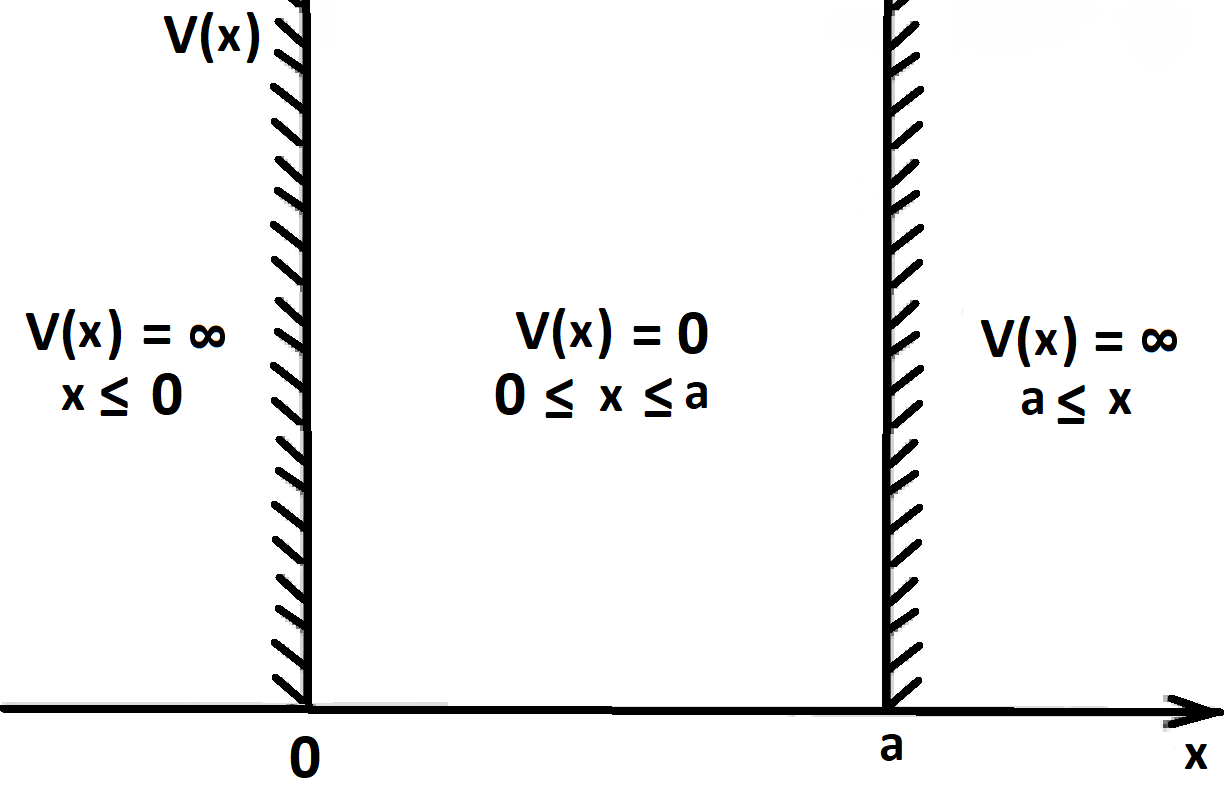
\includegraphics[scale=.65]{infinite_well.png}
\caption{Sonsuz kuyu}
\label{fig:infinite_well}
\end{figure}
%%
Tek boyutlu böyle bir kuyu Schrödinger denklemine,
%%
\begin{equation}
V ( x ) = \left\{
\begin{array} { c l } 
{ \infty } & { \Leftarrow x \leq 0 , x \geq a } \\ 
{ 0 } & { \Leftarrow 0 < x < a } \end{array} 
\right.
\label{eq:infinite_well}
\end{equation}
%%
potansiyelinin konmasıyla tanımlanabilir. Parçacık $0<x<a$ aralığında hapsolduğundan parçacığın dalga fonksiyonu kuyu sınırlarında ve dışında sıfır olmalıdır,
%%
\begin{align*} 
u ( x ) &= 0 \quad x \leq 0 \\ 
u ( x ) &= 0 \quad x \geq a .
\end{align*}
%%
Problemin doğasından ortaya çıkan bu şartlar \emph{sınır şartları} olarak adlandırılır. Kutu dışındaki her yerde dalga fonksiyonu sıfır olduğundan kutunun dışı için Schrödinger denklemi yazılamaz. Kutunun içi içinse $V(x)=0$ olduğundan, birazcık matematiksel düzenlemeyle, Schrödinger denklemi,
%%
\begin{equation}
\frac { d ^ { 2 } u ( x ) } { d x ^ { 2 } } + \frac { 2 m E } { \hbar ^ { 2 } } u ( x ) = 0
\label{eq:infinite_well_schrodinger}
\end{equation}
%%
olarak yazılılır.

\newpage
% In the preamble, add "\renewcommand\refname{New Title}" for article type documents 
% and "\renewcommand\bibname{New Title}" for book and report type documents.
\renewcommand\refname{Kaynaklar}
\bibliography{quantumBIB}{}
%% https://www.sharelatex.com/learn/latex/bibtex_bibliography_styles
 \bibliographystyle{plain}
%% \bibliographystyle{alpha}
%%\bibliographystyle{apalike}
\end{document}

